\documentclass[a1paper,portrait, fontscale=0.45]{baposter}
%\documentclass[a4shrink,portrait,final]{baposter}
% Usa a4shrink for an a4 sized paper.

\tracingstats=2

\usepackage{times}
\usepackage{calc}
\usepackage{graphicx}
\usepackage{amsmath}
\usepackage{amssymb}
\usepackage{relsize}
\usepackage{multirow}
\usepackage{bm}
\usepackage{pgfpages}

%\usepackage{harvard}
%\citationmode{abbr} % forces use of et al all the time (normally only after first one is full cite)
%\renewcommand{\refname}{} % removes the auto inserted "References" header
\usepackage[labelfont=bf]{caption}
%\usepackage[backend = biber]{biblatex}
\usepackage[style=authoryear,maxcitenames = 2,mincitenames = 1,maxbibnames = 99,minbibnames = 1,dashed = false,backend=biber]{biblatex}
\addbibresource{bdrt.bib}
\renewcommand*{\bibfont}{\scriptsize}
\defbibheading{bibliography}[\refname]{}

% This sets the default font to be sans serif
\renewcommand{\familydefault}{\sfdefault}

\usepackage{graphicx}
\usepackage{multicol}
\usepackage{float}

\usepackage{pgfbaselayers}
\pgfdeclarelayer{background}
\pgfdeclarelayer{foreground}
\pgfsetlayers{background,main,foreground}

\usepackage{helvet}
%\usepackage{bookman}
\usepackage{palatino}

% Added by Louis
\usepackage{wrapfig}
\usepackage{enumerate}
\usepackage{arydshln} % for dashed lines
%\linespread{1.2}
% End added by Louis

%\newcommand{\captionfont}{\footnotesize}
\usepackage[font={scriptsize}]{caption}
\selectcolormodel{cmyk}

\graphicspath{{images/}}

%%%%%%%%%%%%%%%%%%%%%%%%%%%%%%%%%%%%%%%%%%%%%%%%%%%%%%%%%%%%%%%%%%%%%%%%%%%%%%%%
%%%% Some math symbols used in the text
%%%%%%%%%%%%%%%%%%%%%%%%%%%%%%%%%%%%%%%%%%%%%%%%%%%%%%%%%%%%%%%%%%%%%%%%%%%%%%%%
% Format 
\newcommand{\Matrix}[1]{\begin{bmatrix} #1 \end{bmatrix}}
\newcommand{\Vector}[1]{\Matrix{#1}}
\newcommand*{\SET}[1]  {\ensuremath{\mathcal{#1}}}
\newcommand*{\MAT}[1]  {\ensuremath{\mathbf{#1}}}
\newcommand*{\VEC}[1]  {\ensuremath{\bm{#1}}}
\newcommand*{\CONST}[1]{\ensuremath{\mathit{#1}}}
\newcommand*{\norm}[1]{\mathopen\| #1 \mathclose\|}% use instead of $\|x\|$
\newcommand*{\abs}[1]{\mathopen| #1 \mathclose|}% use instead of $\|x\|$
\newcommand*{\absLR}[1]{\left| #1 \right|}% use instead of $\|x\|$

\def\norm#1{\mathopen\| #1 \mathclose\|}% use instead of $\|x\|$
\newcommand{\normLR}[1]{\left\| #1 \right\|}% use instead of $\|x\|$

% Some time saving macros
\newcommand{\xit}[1]{x_{#1:t}}
\newcommand{\yit}[1]{y_{#1:t}}
\newcommand{\zit}[1]{z_{#1:t}}

\newcommand{\xik}[1]{x_{#1, k}}
\newcommand{\yik}[1]{y_{#1, k}}
\newcommand{\zik}[1]{z_{#1, k}}
\newcommand{\vik}[1]{\textit{v}_{#1, k}}
\newcommand{\wik}[1]{\textit{w}_{#1, k}}
\newcommand{\mik}[1]{\mu_{#1, k}}
\newcommand{\Sik}[1]{\Sigma_{#1, k}}
\newcommand{\Vk}[1]{V_#1}
\newcommand{\Wk}[1]{W_#1}
\newcommand{\kt}{K_T}
\newcommand{\la}{\lambda_a}
\newcommand{\ls}{\lambda_s}
\newcommand{\lt}{\lambda_{\eta}}
\newcommand{\lei}[1]{\lambda_{\eta_{#1}}}
\newcommand{\tet}{\eta_{x, T}}
\newcommand{\Ik}[1]{\operatorname{I_{#1, k}}}

\newcommand{\ivk}[1]{V_{#1}^{-1}}
\newcommand{\iwk}[1]{W_{#1}^{-1}}

\newcommand{\vk}{V_k}
\newcommand{\wk}{W_k}

\DeclareMathOperator{\giv}{\, | \,}

\DeclareMathOperator{\lint}{\displaystyle\int}
\DeclareMathOperator{\lprod}{\displaystyle\prod}

\DeclareMathSizes{6}{5}{3}{2}

%%%%%%%%%%%%%%%%%%%%%%%%%%%%%%%%%%%%%%%%%%%%%%%%%%%%%%%%%%%%%%%%%%%%%%%%%%%%%%%%
% Multicol Settings
%%%%%%%%%%%%%%%%%%%%%%%%%%%%%%%%%%%%%%%%%%%%%%%%%%%%%%%%%%%%%%%%%%%%%%%%%%%%%%%%
\setlength{\columnsep}{0.7em}
\setlength{\columnseprule}{0mm}


%%%%%%%%%%%%%%%%%%%%%%%%%%%%%%%%%%%%%%%%%%%%%%%%%%%%%%%%%%%%%%%%%%%%%%%%%%%%%%%%
% Save space in lists. Use this after the opening of the list
%%%%%%%%%%%%%%%%%%%%%%%%%%%%%%%%%%%%%%%%%%%%%%%%%%%%%%%%%%%%%%%%%%%%%%%%%%%%%%%%
\newcommand{\compresslist}{%
\setlength{\itemsep}{1pt}%
\setlength{\parskip}{0pt}%
\setlength{\parsep}{0pt}%
}


%%%%%%%%%%%%%%%%%%%%%%%%%%%%%%%%%%%%%%%%%%%%%%%%%%%%%%%%%%%%%%%%%%%%%%%%%%%%%%
%%% Begin of Document
%%%%%%%%%%%%%%%%%%%%%%%%%%%%%%%%%%%%%%%%%%%%%%%%%%%%%%%%%%%%%%%%%%%%%%%%%%%%%%

\begin{document}

%%%%%%%%%%%%%%%%%%%%%%%%%%%%%%%%%%%%%%%%%%%%%%%%%%%%%%%%%%%%%%%%%%%%%%%%%%%%%%
%%% Here starts the poster
%%%---------------------------------------------------------------------------
%%% Format it to your taste with the options
%%%%%%%%%%%%%%%%%%%%%%%%%%%%%%%%%%%%%%%%%%%%%%%%%%%%%%%%%%%%%%%%%%%%%%%%%%%%%%
% Define some colors
\definecolor{silver}{cmyk}{0,0,0,0.3}
\definecolor{yellow}{cmyk}{0,0,0.9,0.0}
\definecolor{reddishyellow}{cmyk}{0,0.22,1.0,0.0}
\definecolor{black}{cmyk}{0,0,0.0,1.0}
\definecolor{darkYellow}{cmyk}{0,0,1.0,0.5}
\definecolor{darkSilver}{cmyk}{0,0,0,0.1}

\definecolor{lightyellow}{cmyk}{0,0,0.3,0.0}
\definecolor{lighteryellow}{cmyk}{0,0,0.1,0.0}
\definecolor{lighteryellow}{cmyk}{0,0,0.1,0.0}
\definecolor{lightestyellow}{cmyk}{0,0,0.05,0.0}

\definecolor{tcdblue}{RGB}{0,114,198} % This is the officially recognised TCD blue, as defined on the TCD website
\definecolor{tcdgrey}{RGB}{83,86,90}  % This is the officially recognised TCD grey, as defined on the TCD website


%%
\typeout{Poster Starts}
\background{
  \begin{tikzpicture}[remember picture,overlay]%
    \draw (current page.north west)+(-2em,2em) node[anchor=north west] {\includegraphics[height=1.1\textheight]{background}};
  \end{tikzpicture}%
}

\newlength{\leftimgwidth}
\begin{poster}%
  % Poster Options
  {
  % Show grid to help with alignment
  grid=false,
  % Column spacing
  colspacing=1em,
  % Color style
  bgColorOne=white,
  bgColorTwo=white,
  borderColor=tcdblue,
  headerColorOne=white,
  headerColorTwo=white,
  headerFontColor=tcdblue,
  boxColorOne=white,
  boxColorTwo=white,
  % Format of textbox
  textborder=rectangle,
  % Format of text header
  eyecatcher=true,
  headerborder=open,
  headerheight=9em, %0.12\textheight,
  headershape=rectangle,
  headershade=plain,
  headerfont=\normalsize,
  boxshade=plain,
%  background=shade-tb,
  background=plain,
  linewidth=1pt
  }
  % Eye Catcher
  {
\includegraphics[height=8em]{trinity-stacked.jpg}}
  % Title 
  {
  {\Huge Bayesian Dynamic Regression Trees} \\
  {\Large Inference and Learning for Streaming Data}
  }
  % Authors
  {  
  {\large Michael Ferreira {\smaller (ferreima@tcd.ie)}} {\large and Simon P Wilson {\smaller (swilson@tcd.ie)}}
  
  \vspace{0.2em}
  {\large Trinity College Dublin}
  }
  % University and sponsor logos
  {
      \begin{minipage}{9em}
       \hfill
        
\includegraphics[height=5em]{insight.png}
        % \hfill
        
\includegraphics[height=5em]{SFI_logo_stacked_en.jpg}
         % \hfill
      \end{minipage}
  }

  \tikzstyle{light shaded}=[top color=baposterBGtwo!30!white,bottom color=baposterBGone!30!white,shading=axis,shading angle=30]

  % Width of left inset image
   \setlength{\leftimgwidth}{0.78em+8.0em}

%%%%%%%%%%%%%%%%%%%%%%%%%%%%%%%%%%%%%%%%%%%%%%%%%%%%%%%%%%%%%%%%%%%%%%%%%%%%%%
%%% Now define the boxes that make up the poster
%%%---------------------------------------------------------------------------
%%% Each box has a name and can be placed absolutely or relatively.
%%% The only inconvenience is that you can only specify a relative position 
%%% towards an already declared box. So if you have a box attached to the 
%%% bottom, one to the top and a third one which should be in between, you 
%%% have to specify the top and bottom boxes before you specify the middle 
%%% box.
%%%%%%%%%%%%%%%%%%%%%%%%%%%%%%%%%%%%%%%%%%%%%%%%%%%%%%%%%%%%%%%%%%%%%%%%%%%%%%
    %
    % A coloured circle useful as a bullet with an adjustably strong filling
    \newcommand{\colouredcircle}[1]{%
      \tikz{\useasboundingbox (-0.2em,-0.32em) rectangle(0.2em,0.32em); \draw[draw=black,fill=baposterBGone!80!black!#1!white,line width=0.03em] (0,0) circle(0.18em);}}

%%%%%%%%%%%%%%%%%%%%%%%%%%%%%%%%%%%%%%%%%%%%%%%%%%%%%%%%%%%%%%%%%%%%%%%%%%%%%%
\headerbox{1. Contribution}{name=contribution,column=0,row=0}{
%%%%%%%%%%%%%%%%%%%%%%%%%%%%%%%%%%%%%%%%%%%%%%%%%%%%%%%%%%%%%%%%%%%%%%%%%%%%%%
	\small{We introduce a flexible system of modelling streaming data in a Bayesian regression setting. We combine two regression methods, Bayesian Cart by \cite{bcart} and the Kalman Filter as derived by \cite{singpur} because both minimise the mean square error based on the conditional expectation. Like \cite{bart} we form an ensemble of trees and perform inference over the weighted sum of the trees. Similar work has been done by \cite{taddy} and \cite{gramacy}. }
}

%%%%%%%%%%%%%%%%%%%%%%%%%%%%%%%%%%%%%%%%%%%%%%%%%%%%%%%%%%%%%%%%%%%%%%%%%%%%%%
  \headerbox{References}{name=refs,column=0,span=1,above=bottom}{
%%%%%%%%%%%%%%%%%%%%%%%%%%%%%%%%%%%%%%%%%%%%%%%%%%%%%%%%%%%%%%%%%%%%%%%%%%%%%%
\printbibliography
}

%%%%%%%%%%%%%%%%%%%%%%%%%%%%%%%%%%%%%%%%%%%%%%%%%%%%%%%%%%%%%%%%%%%%%%%%%%%%%%
  \headerbox{2. Trees and Filters}{name=TandF,column=0,span=1,below=contribution,above=refs}{
%%%%%%%%%%%%%%%%%%%%%%%%%%%%%%%%%%%%%%%%%%%%%%%%%%%%%%%%%%%%%%%%%%%%%%%%%%%%%%
\small{A tree divides up a large covariate space, $\bm{\mathcal{X}}$, using splitting threshold rules which assign observations to each of the partitions. This provides both a prior structure on the covariate space and concentrates the likelihood of the observations to each partition based on the conditional expectation: $E[y_t \giv X_{t,i} \dots\ X_{t, i+j}] = z_t$}
\begin{figure}[H]
\hspace{1em}
\begin{minipage}[c]{0.42\linewidth}
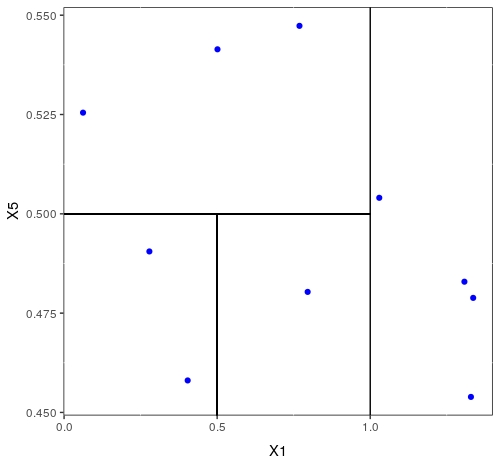
\includegraphics[width=\linewidth]{tree1.jpeg}
\label{fig:xparts1}
\end{minipage}
\hspace{1.5em}
\begin{minipage}[c]{0.42\linewidth}
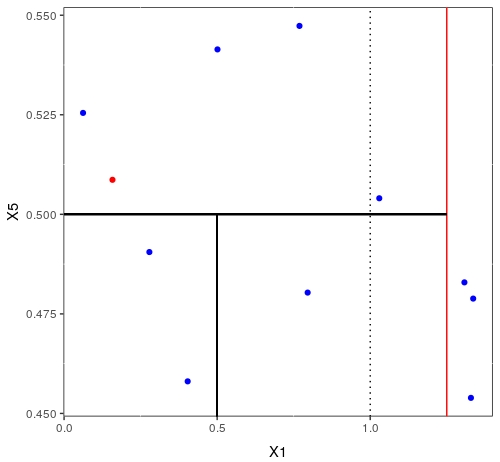
\includegraphics[width=\linewidth]{tree2.jpeg}
\label{fig:xparts2}
\end{minipage}
\vspace{-1em}
\caption{An evolving tree space.}
\end{figure}

\small{The Kalman filter prediction of the next observation is based on the conditional expectation of the previous state: $E[y_t \giv z_t] = HFz_{t-1}$, where $y_t = Hz_t + v_t$ and $z_t = Fz_{t-1} + w_t$}\\

\small{Using an adaptation of the Kalman filter to a sensor network, \cite{sinopoli} developed an intermittent Kalman filter which we use as a means of updating the $1 \dots K_T$ filters of each tree.} 
%\vspace{-1em}
\begin{figure}[H]
\hspace{1em}
\begin{minipage}[c]{0.42\linewidth}
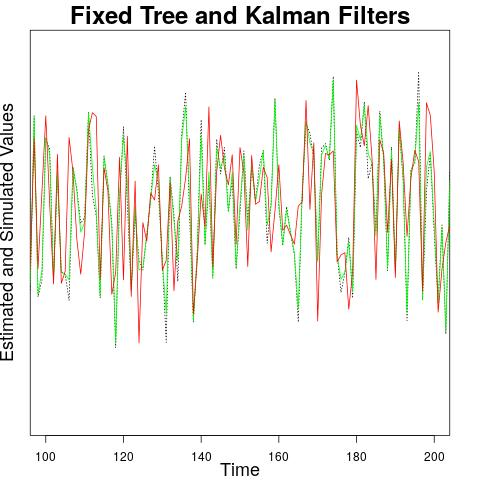
\includegraphics[width=\linewidth]{fixkf.jpeg}
\label{fig:fixtree1}
\end{minipage}
\hspace{1.5em}
\begin{minipage}[c]{0.42\linewidth}
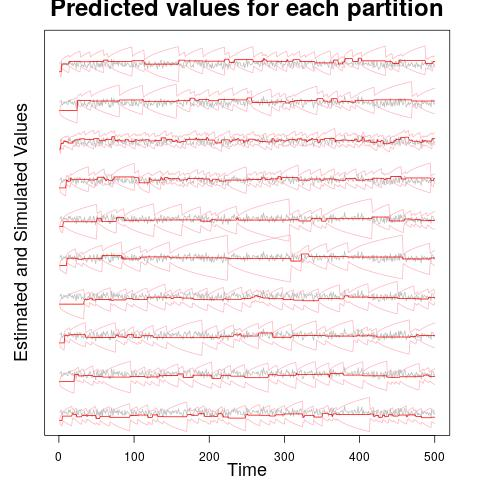
\includegraphics[width=\linewidth]{fixpred.jpeg}
\label{fig:fixtree2}
\end{minipage}
\vspace{-1.7em}
\caption{Estimating a process by creating smaller subprocesses.}
\end{figure}

In Bayesian dynamic regression trees (BDRT) a stream of data $(x_t, y_t)$ is considered, with $y_t$ following the regression tree model as described in Section 3. The latent mean process is dynamic as is the growth of the tree structure. This permits the relationship between $y_t$ and $x_t$ to change with time as the relationship between $y_t$ and $z_t$ is changing. Each leaf then models an independent Gaussian process.
}
%%%%%%%%%%%%%%%%%%%%%%%%%%%%%%%%%%%%%%%%%%%%%%%%%%%%%%%%%%%%%%%%%%%%%%%%%%%%%%
\headerbox{3. Base Model}{name=bm,column=1,span=1,row=0}{
%%%%%%%%%%%%%%%%%%%%%%%%%%%%%%%%%%%%%%%%%%%%%%%%%%%%%%%%%%%%%%%%%%%%%%%%%%%%%%
\small{Let $y_t \in \mathbb{R}^n$ and $x_t \in \mathbb{R}^m$.  The tree $T$ partitions ${\cal X} \subseteq \mathbb{R}^p$ into $K_T$ subsets (e.g.\ it has $K_T$ leaves), so $z_t = (z_{t1},\ldots,z_{tK_T})$, with $z_{tk} \in \mathbb{R}^m$. Then we describe the model as follows:
\begin{flalign}
&E(y \, | \, T, z, x) \: = \: z_{\eta(x,T)} \\ \nonumber
&y_t \, | \, T, z_t, x_t \: \sim \: N(z_{t,\eta(x_t, T)}, V_{\eta(x_t, T)}) \\ \nonumber
&z_{t+1,k} \: \sim \: N(F_k z_{tk}, W_k), \; k=1,\ldots,K_T \\ \nonumber
\label{eq:rt_def}
\end{flalign}

\vspace{-1.9em}
Thus we have multiple independent autoregressive Gaussian process with initial values $z_{0k} \sim N(\mu_{0k}, W_{0k})$.\\

The $p(z_{tk} \giv T, \theta_T, x^t, y^t)$ is derived from the Kalman filter and the Gaussian model at the partitions allows us to derive an exact form of $p(T \giv \theta_T, x^t, y^t) = $
\vspace{-0.6em}
\begin{flalign*}
&p(T) \lprod^{K_T}_{k = 1} \lint p(\zik{0}) \lprod_{i = 1}^t p(y_i \giv \zik{i}, T)^{\Ik{i}} \\ \nonumber
&\cdot p(\zik{i} \giv \zik{i-1}, u_t, T) dz^t_k \\ \nonumber
 &=p(T)\lprod^{K_T}_{k = 1}(|2\pi W_0|)^{-\frac{1}{2}} \\ \nonumber
&\cdot \left(\lprod_{i = 1}^t(|2\pi\wk ||2\pi A_i|)^{-\frac{1}{2}}(|2\pi\vk|)^{\frac{-\Ik{i}}{2}}\right)\cdot \\
 &\exp \bigg[-\frac{1}{2} \biggl(\mik{0}\iwk{0}\mik{0} - d_0^TA_i^{-1}d_0 + \\ \nonumber 
 &\sum_{i = 1}^t \Ik{i} \yik{i}^T\ivk{k}\yik{i} + u_{i}^TG^T\iwk{k}Gu_{i} - d_i^TA_i^{-1}d_i \biggr) \bigg]. && 
\end{flalign*} 

\vspace{-0.5em}
The main point to note is that this computation is $O(n)$ because the current term only relies on the previous term. Thus the the main factors influencing complexity are the Kalman filter, $O(n^3)$ and tree size. Using Openmp we get $O(\lceil r \max(K_T)/P \rceil n^3)$ for each iteration of $r$ trees.}
}

%%%%%%%%%%%%%%%%%%%%%%%%%%%%%%%%%%%%%%%%%%%%%%%%%%%%%%%%%%%%%%%%%%%%%%%%%%%%%%
\headerbox{4. Simulation Study}{name=ss,column=1,span=2, above=bottom}{
%%%%%%%%%%%%%%%%%%%%%%%%%%%%%%%%%%%%%%%%%%%%%%%%%%%%%%%%%%%%%%%%%%%%%%%%%%%%%%
BDRT are:w
 compared to the Kalman Filter. \small{A time-series data set was simulated using the Mackey-Glass non-linear time series with a $\tau$ of 20. 50 trees over 100 iterations were used with known parameters:
\begin{align*}
H = 
\begin{bmatrix}
1 \\ 1
\end{bmatrix}, \quad
F = 
\begin{bmatrix}
0.9 & 0 \\ 0 & 0.2
\end{bmatrix}, \quad
W = 
\begin{bmatrix}
0.1 & 0 \\ 0 & 0.1
\end{bmatrix}, \quad
y \in \mathbb{R}, \quad z \in \mathbb{R}^2 \quad \text{and} \quad V = 0.03.
\end{align*}
}
\begin{multicols}{3}
\begin{figure}[H]
\hspace{1em}
\begin{minipage}[c]{0.6\linewidth}
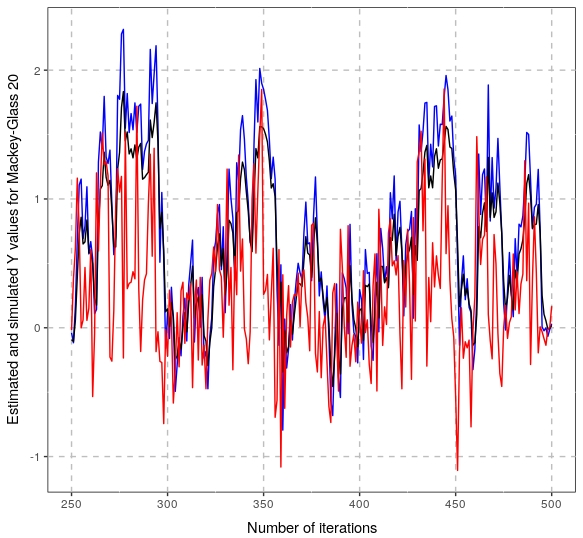
\includegraphics[width=\linewidth]{statey.jpeg}
\label{fig:ypred}
\vspace{-1.7em}
\caption{Showing observation predictions with BDRT and the Kalman Filter}
\end{minipage}
\end{figure}
\begin{figure}[H]
\hspace{1em}
\begin{minipage}[c]{0.6\linewidth}
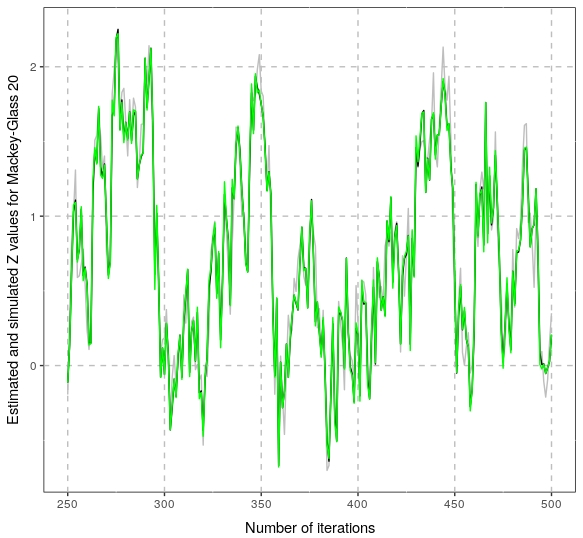
\includegraphics[width=\linewidth]{statez.jpeg}
\label{fig:zpred}
\vspace{-1.7em}
\caption{Showing latent state predictions with BDRT and the Kalman Filter}
\end{minipage}
\end{figure}
\begin{figure}[H]
\hspace{1em}
\begin{minipage}[c]{0.6\linewidth}
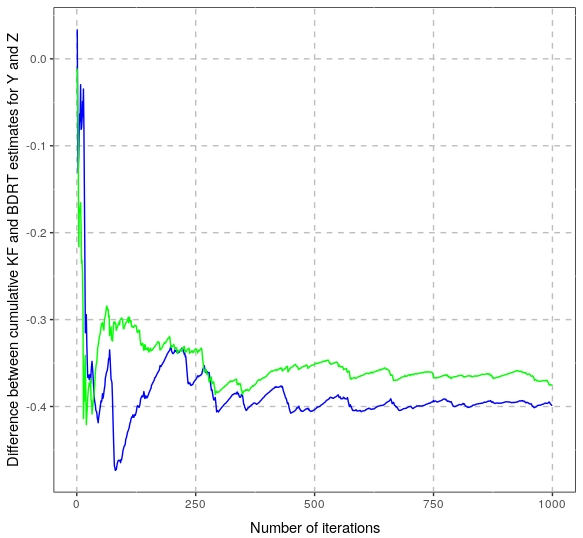
\includegraphics[width=\linewidth]{kbdiff.jpeg}
\label{fig:kbdiff}
\vspace{-1.7em}
\caption{Difference in RMSE between BDRT and the Kalman Filter}
\end{minipage}
\end{figure}
\end{multicols}
Comparing different MCMC methods on BDRT. \small{"MH" is the Chipman et al. method using grow, prune, swap and change. "BST" uses the same moves but has 10 levels of heating. The pseudoprior is estimated stochastically using the method suggested by \cite{geyer}. "MST" uses different moves: multigrow, multiprune, multichange, shift, and swap. The upper bound of growing, changing and pruning is temperature dependent.}
\begin{multicols}{3}
\begin{figure}[H]
\hspace{1em}
\begin{minipage}[c]{0.6\linewidth}
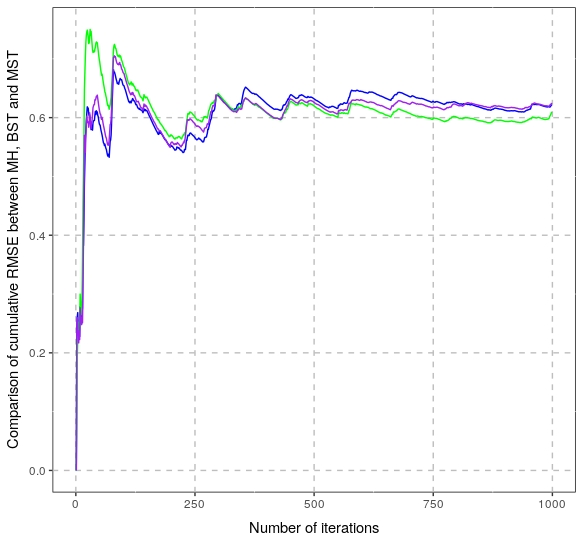
\includegraphics[width=\linewidth]{comp3rmse.jpeg}
\label{fig:comprmse}
\vspace{-1.7em}
\caption{Comparing RMSE between the 3 different MCMC approaches.}
\end{minipage}
\end{figure}
\begin{figure}[H]
\hspace{1em}
\begin{minipage}[c]{0.6\linewidth}
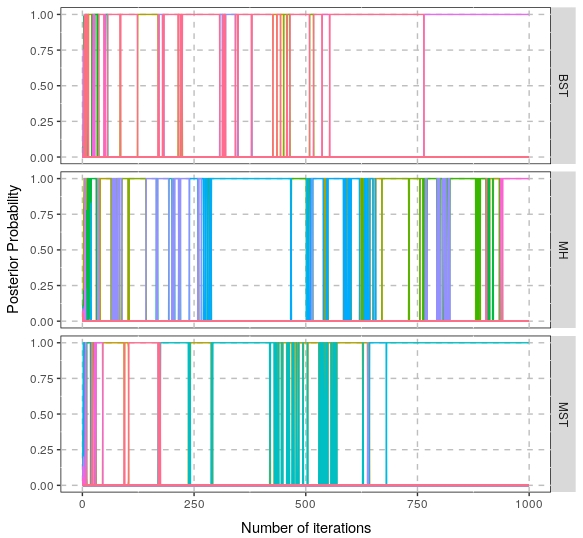
\includegraphics[width=\linewidth]{comp3postmix.jpeg}
\label{fig:comppost}
\vspace{-1.7em}
\caption{The probability of the trees alternate between zero and one.}
\end{minipage}
\end{figure}
\begin{figure}[H]
\hspace{1em}
\begin{minipage}[c]{0.6\linewidth}
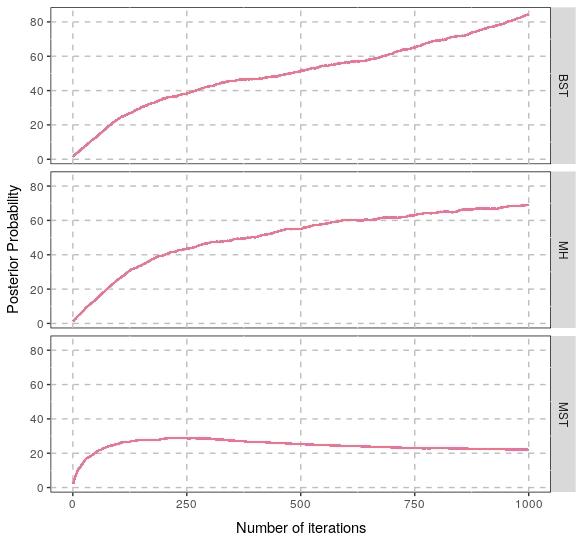
\includegraphics[width=\linewidth]{comp3treesize.jpeg}
\label{fig:compsize}
\vspace{-1.7em}
\caption{Average tree size as the algorithm progresses}
\end{minipage}
\end{figure}
\begin{figure}[H]
\hspace{1em}
\begin{minipage}[c]{0.6\linewidth}
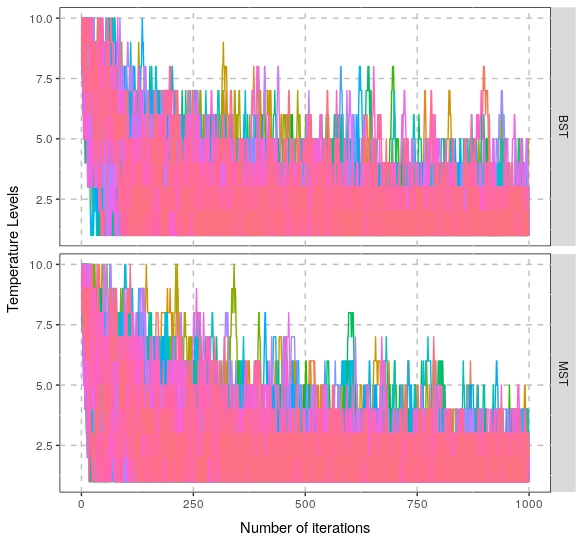
\includegraphics[width=\linewidth]{comp2levels.jpeg}
\label{fig:compsimtem}
\vspace{-1.7em}
\caption{Temperature traversal of the trees started at the highest temperature.}
\end{minipage}
\end{figure}
\begin{figure}[H]
\hspace{1em}
\begin{minipage}[c]{0.6\linewidth}
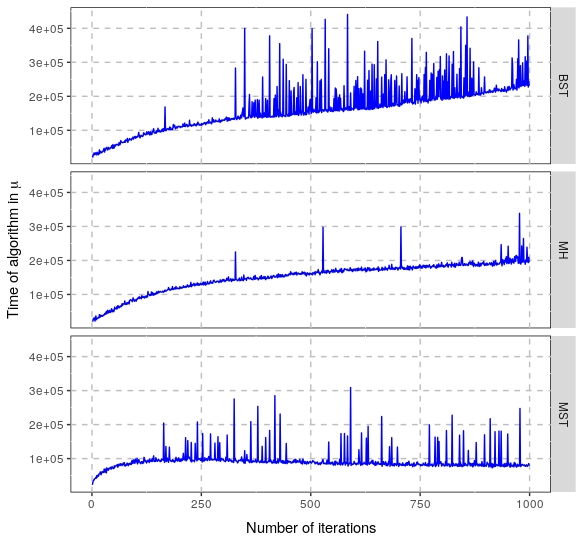
\includegraphics[width=\linewidth]{comp3times.jpeg}
\label{fig:comptimes}
\vspace{-1.7em}
\caption{Time comparisons between different MCMC methods.}
\end{minipage}
\end{figure}
\begin{figure}[H]
\hspace{1em}
\begin{minipage}[c]{0.6\linewidth}
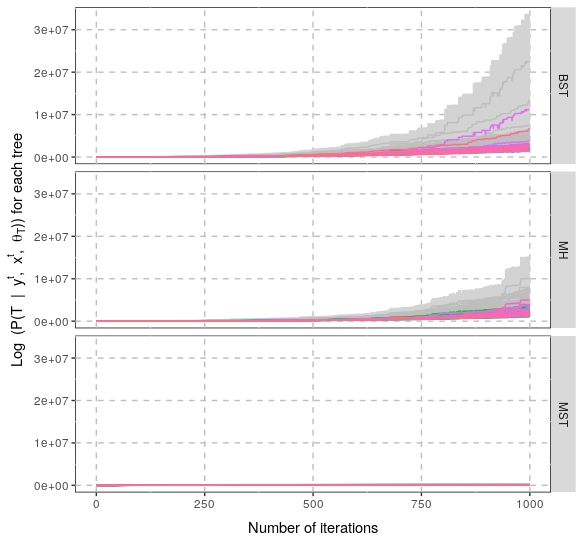
\includegraphics[width=\linewidth]{comp3qstar.jpeg}
\label{fig:comptimes}
\vspace{-1.7em}
\caption{The log posterior for updated and not-updated leaves and their sum.}
\end{minipage}
\end{figure}
\end{multicols}
}

%%%%%%%%%%%%%%%%%%%%%%%%%%%%%%%%%%%%%%%%%%%%%%%%%%%%%%%%%%%%%%%%%%%%%%%%%%%%%%
\headerbox{5. Streaming}{name=stream,column=2,row=0,span=1}{
%%%%%%%%%%%%%%%%%%%%%%%%%%%%%%%%%%%%%%%%%%%%%%%%%%%%%%%%%%%%%%%%%%%%%%%%%%%%%%
\small{Exchangeability of responses based on conditional data allows us to to develop a window-like streaming algorithm. If the data is arriving faster than it can be processed, $\lambda_a < \lambda_s$, then we can randomly select inputs within the window size and discard/store those that preceded the selected input. \\

The size of the window is based on the decisions and resources available to the analyst including,
tree size ($K_T$), rate of data arrival, ($\lambda_s$), rate of algorithm ($\lambda_a$), choice of model type (state only estimation, dual estimation, parameter learning, variable or model selection).}
}

%%%%%%%%%%%%%%%%%%%%%%%%%%%%%%%%%%%%%%%%%%%%%%%%%%%%%%%%%%%%%%%%%%%%%%%%%%%%%%
\headerbox{6. Extensions and More}{name=extend,column=2,span=1,below=stream,above=ss}{
%%%%%%%%%%%%%%%%%%%%%%%%%%%%%%%%%%%%%%%%%%%%%%%%%%%%%%%%%%%%%%%%%%%%%%%%%%%%%%
\small{One of the reasons for using the Kalman Filter is that many extensions exist. In particular, the Unscented Kalman filter allows for nonlinear dynamics to be modelled and is an improvement over the Extended Kalman Filter. The calculation of the posterior uses the idea that the marginalisation over $z_t$ in the posterior calculation is the same as the expectation w.r.t. $z_t$ and $p(T \giv \theta_T, x^t, y^t)$.\\

\vspace{-0.5em}
There are also methods developed by \cite{mehra} and others that allow us to adapt the algorithm for inference on the variance of the state $W_t$. \\

\vspace{-0.5em}
A further adaptation under development is to declare each leaf as a Gaussian marginal so that each tree represents a Gaussian process, i.e. the leaves of the tree represent the components of a vector $\in \mathbb{R}^{|K_T|}$ where each leaf may be $\in \mathbb{R}^m$. In this case we have fixed tree sizes.}
}

\end{poster}
\end{document}
